\documentclass{standalone}
\usepackage{pgfplots}
\pgfplotsset{compat=1.18}

\begin{document}

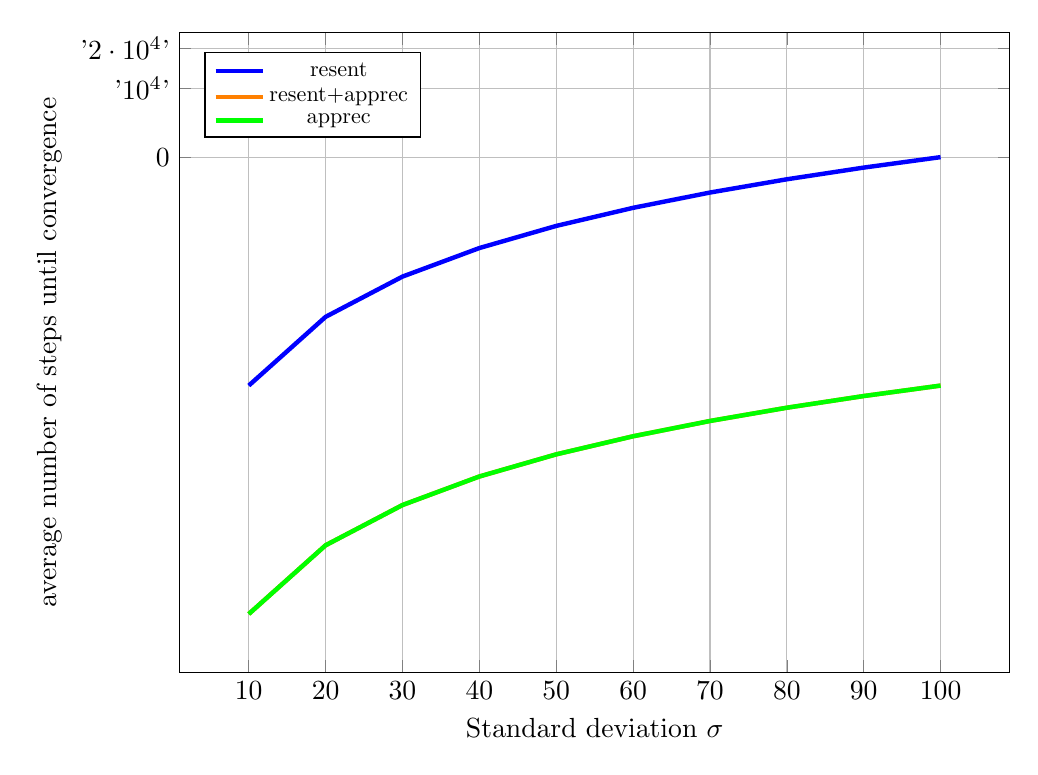
\begin{tikzpicture}
    \begin{axis}[
        width=\textwidth,
        height=0.8\textwidth,
        xlabel={Standard deviation $\sigma$},
        ylabel={average number of steps until convergence},
        ymin=0,
        ymax=35000,
        ytick={0, 10000, 20000, 30000},
        yticklabels={$0$, '$10^4$', '$2\cdot10^4$', '$3\cdot10^4$'},
        legend pos=north west,
        grid=major,
        legend style={nodes={scale=0.8, transform shape}},
        log basis y={10},
        ymode=log,
        xmajorgrids=true,
        ymajorgrids=true,
        every axis plot/.append style={ultra thick},
        ]
        \addplot[blue,mark=none] coordinates {
            (0, 0)
            (10, 1000)
            (20, 2000)
            (30, 3000)
            (40, 4000)
            (50, 5000)
            (60, 6000)
            (70, 7000)
            (80, 8000)
            (90, 9000)
            (100, 10000)
        };
        \addlegendentry{resent}

        \addplot[orange,mark=none] coordinates {
            (0, 0)
            (10, 100)
            (20, 200)
            (30, 300)
            (40, 400)
            (50, 500)
            (60, 600)
            (70, 700)
            (80, 800)
            (90, 900)
            (100, 1000)
        };
        \addlegendentry{resent+apprec}

        \addplot[green,mark=none] coordinates {
            (0, 0)
            (10, 100)
            (20, 200)
            (30, 300)
            (40, 400)
            (50, 500)
            (60, 600)
            (70, 700)
            (80, 800)
            (90, 900)
            (100, 1000)
        };
        \addlegendentry{apprec}
    \end{axis}
\end{tikzpicture}

\end{document}